\documentclass[20pt,margin=1in,innermargin=-4.5in,blockverticalspace=-0.25in]{tikzposter}
\geometry{paperwidth=48in,paperheight=36in}
\usepackage[utf8]{inputenc}
\usepackage{amsmath}
\usepackage{amsfonts}
\usepackage{amsthm}
\usepackage{amssymb}
\usepackage{mathrsfs}
\usepackage{graphicx}
\usepackage{adjustbox}
\usepackage{enumitem}
\usepackage[backend=biber,style=numeric]{biblatex}
\usepackage{emory-theme}

\usepackage{mwe} % for placeholder images

\addbibresource{refs.bib}

% set theme parameters
\tikzposterlatexaffectionproofoff
\usetheme{EmoryTheme}
\usecolorstyle{EmoryStyle}

\title{ETERNITY:NUMBERS}
\author{SARGUN KAUR DHANJU}
\institute{CONCORDIA UNIVERSITY\\
            }
\titlegraphic{
\includegraphics[width=0.1\textwidth]{CONCORDIA.jpg}}

% begin document
\begin{document}
\maketitle
\centering
\begin{columns}
    \column{0.32}
    \block{Description}{
    \vspace{2cm}
         In this project, I had to build a calculator, that apart from performing basic computations, calculated the value of pi and has buttons to perform simple pi related calculations such as Area, Perimeter, etc.
         \begin{tikzfigure}
            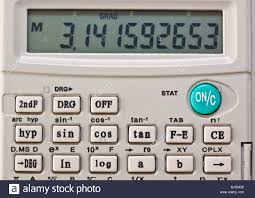
\includegraphics[width=0.8\linewidth]{download.jpg}
        \end{tikzfigure}
    \vspace{4cm}
    }
    \block{What Worked Well?}
    {
    \vspace{2cm}
    \begin{tikzfigure}
            
\includegraphics[width=0.4\linewidth]{well.jpg}
        \end{tikzfigure}
    \begin{itemize}
        \item Team coordination was excellent whenever it was needed. All the team members were very helpful.
        \item Realization of self confidence as I had to complete all the tasks by myself.
        \item Timely completion of each deliverable.
        \item Working on pi was easy as it is the most commonly occurring irrational number.
        \item Got an excellent interviewee for this project.
    \end{itemize}
    \vspace{2cm}
   }
    \block{Challenges Faced}{
       \vspace{1cm}
       \begin{tikzfigure}
            
\includegraphics[width=0.4\linewidth]{challenges.jpg}
        \end{tikzfigure}
       \begin{itemize}
           \item I worked on latex for the first time, so it was quite time consuming.
           \item Managing time for the project.
           \item Different time zone of the interviewee.
           \item Deciding a template for poster.
       \end{itemize}
       }
    \column{0.36}
    \block{What Can Be Improved?}
    {
    \vspace{0.5cm}
        \begin{itemize}
            \item Implementation- the computation can be performed on two numbers for now.
            \item Number of user stories could have been more.
            \begin{tikzfigure}
            
\includegraphics[width=0.28\linewidth]{improve.jpg}
        \end{tikzfigure}
            \item There could have been more team oriented tasks so that there could be a feeling of oneness among the team members.
            \item Proficiency in latex.
        \end{itemize}
       \vspace{2cm}
        \begin{tikzfigure}
            
\includegraphics[width=0.9\linewidth]{pi_.jpg}
        \end{tikzfigure}
        \vspace{2cm}
        Though pi is a very common irrational number, but while working on this project, I got to know many facts about it that I would have never known otherwise. I got to know that this number is so famous that there is a day to celebrate it. It is an irrational number that is represented as a ratio of two rational numbers.
        \vspace{2cm}
         \begin{tikzfigure}
            
\includegraphics[width=0.9\linewidth]{images.jpg}
        \end{tikzfigure}
    }
    \column{0.32}
   \block{Critical Decisions}
    {
    \begin{itemize}
        \item Choosing the interviewee- Among the 3 available interviewees, I selected the one who had more knowledge about pi.
        \item Selection of persona template- All the team members suggested templates for persona, but we eventually decided to go with a template that could be easily implemented by all the team members.
        \item Designing interview questions- I made a lot of interview questions initially, but before conducting the interview, I eliminated irrelevant questions.
    \end{itemize}
     \begin{tikzfigure}
            
\includegraphics[width=0.4\linewidth]{decision.jpg}
        \end{tikzfigure}
        }
    
     \block{Lessons Learnt}{
    \begin{itemize}
        \item Preparing document in Latex.
        \item Working individually could be fun.
        \item Time management.
    \end{itemize}
        
        \begin{tikzfigure}
            
\includegraphics[width=0.5\linewidth]{lesson.jpg}
        \end{tikzfigure}
    }
     \block{References}{
        \vspace{1cm}
       
         [1]\textbf{ }P. Kamthan, Summer 2019, $``$Project Description$"$ , Department of Computer Science and Software Engineering, Concordia University.
         
         
         
         
         [2]\textbf{ }Barcode Generator. Available: https://www.cognex.com/en-ca/resources/interactive-tools/free-barcode-generator
         \vspace{1cm}
         
         
         
         Github-
         \begin{tikzfigure}
            
\includegraphics[width=0.5\linewidth]{Barcode.jpg}
        \end{tikzfigure}
         
        
    }
\end{columns}
\end{document}